\chapter{Task Adaptation in Imitation Learning with \TAIL{} Agent\label{ch:TAIL}}


The previous chapter introduced \DAIL{} agent to tackle the domain adaptation in imitation learning.
In this chapter, the task adaptation problem is then focused on.
The \TAIL{} agent is introduced to address the problem.

\renewcommand{\SectionsDir}{Chapter4/Sections}
\renewcommand{\FigsDir}{Chapter4/Figs}
\renewcommand{\TablesDir}{Chapter4/Tables}


\section{Introduction\label{ch:TAIL:sec:Introduction}}
Imitation learning has been growing in popularity and has achieved some successes in numerous tasks, including robotics control \cite{IL_Robotics_1, IL_Robotics_2, IL_Robotics_3} and autonomous driving \cite{IL_Driving_1, IL_Driving_2, IL_Driving_3, IL_Driving_4}.
Despite certain achievements,
IL agents are designed to focus on accomplishing only a single, narrowly defined task.
Therefore, when given a new task, the agent has to start the learning process again from the ground up, even if it has already learned a task that is related to and shares the same structure with the new one.
% On the other hand,
% humans are capable of efficiently generalizing the learned knowledge and leveraging that to solve such related tasks in a short time.
On the other hand,
humans possess an astonishing ability in the learning process, where the knowledge learned from source tasks can be leveraged for learning a new task.
For example,
an infant can reuse and augment the motor skills obtained when he learns to walk or uses his hand,
for more complex tasks later in his life (e.g., riding a bike).
Transfer learning (TL) is a technique based on this idea.
TL enables the agent to reuse its knowledge learned from a source task in order to facilitate learning a new target task,
resulting in a more generalized agent.


Recent studies have applied TL to RL/IL agents and achieved some success,
especially in robot manipulation tasks since these tasks usually share a common structure (i.e., robot arm) \cite{TL_Robotics_1, TL_Robotics_2, TL_Robotics_3}.
However, transfer learning requires training the agent on the source task first.
Then, the trained agent is adapted to the target task using fine tuning.
Unlike transfer learning,
the \TAIL{} agent is proposed, which utilizes adversarial learning to train and adapt the agent simultaneously.
The evaluation results show that the proposed agent has a better learning performance compared to existing transfer learning
approaches.


\section{Problem Formulation\label{ch:TAIL:sec:ProblemFormulation}}
The task problem in imitation learning can be formalized as an episodic Markov decision process (MDP).
A MDP $\mathbb{M}^-_x$ for a task $x$ with finite time horizon $H_x$ \cite{RL_AnIntroductionBook} is represented as the following equation:
\begin{equation}
  \mathbb{M}^-_x = (\mathcal{S}_x, \mathcal{A}_x, P_x, \gamma, H_x)
\end{equation}
where
$\mathcal{S}_x$ and $\mathcal{A}_x$ represent the continuous state and action spaces, respectively;
$P_x(s'|s,a)$ denotes the transition probability function;
$\gamma$ is the discount factor.
A stochastic policy $\pi_x(s,a)$ for $\mathbb{M}^-_x$
describes a mapping from each state to the probability of taking each action.
The goal of an IL agent is to learn an optimal policy $\pi^{*}_x$ that imitates the expert policy $\hat{\pi}_x$ given demonstrations from that expert.
An expert demonstration for a task $x$ is defined as a sequence of state--action pairs $\tau_{x} = \{(\hat{s}^t_{x}, \hat{a}^t_{x}) : t \in [0, H_x]\}$.
It should be noted that the set of expert demonstrations is collected under different domain and settings.

Let $\mathbb{M}^-_{S}$ denote a source task,
which provides prior knowledge $\mathcal{K}_S$ that is accessible by the target task $\mathbb{M}^-_T$,
such that by leveraging $\mathcal{K}_S$,
the target agent learns better in the target task $\mathbb{M}^-_T$.
The main objective is to learn an optimal policy $\pi^{*}_{T}(\mathcal{K}_S, \mathcal{K}_T)$ for target tasks,
by leveraging $\mathcal{K}_S$ from $\mathbb{M}^-_S$.


\section{The Proposed \TAIL{} Agent\label{ch:TAIL:sec:Proposal}}
In this section, the proposed \TAIL{} agent is introduced.
The architecture of the proposed agent is the same as \DAIL{}, which is illustrated in Figure \ref{ch:TAIL:fig:Architecture}.
It is important to note that the loss functions for three deep feed-forward networks $F$, $G$, and $D$ are similar to the \DAIL{} agent.
The only difference is that the \TAIL{} agent is trained on both source and target tasks simultaneously and under the same domain.
Thus, instead of extracting domain-shared and domain-specific features, \TAIL{} is trained to learn the similarities and differences between source and target tasks.

\begin{figure}[H]
  \centering
  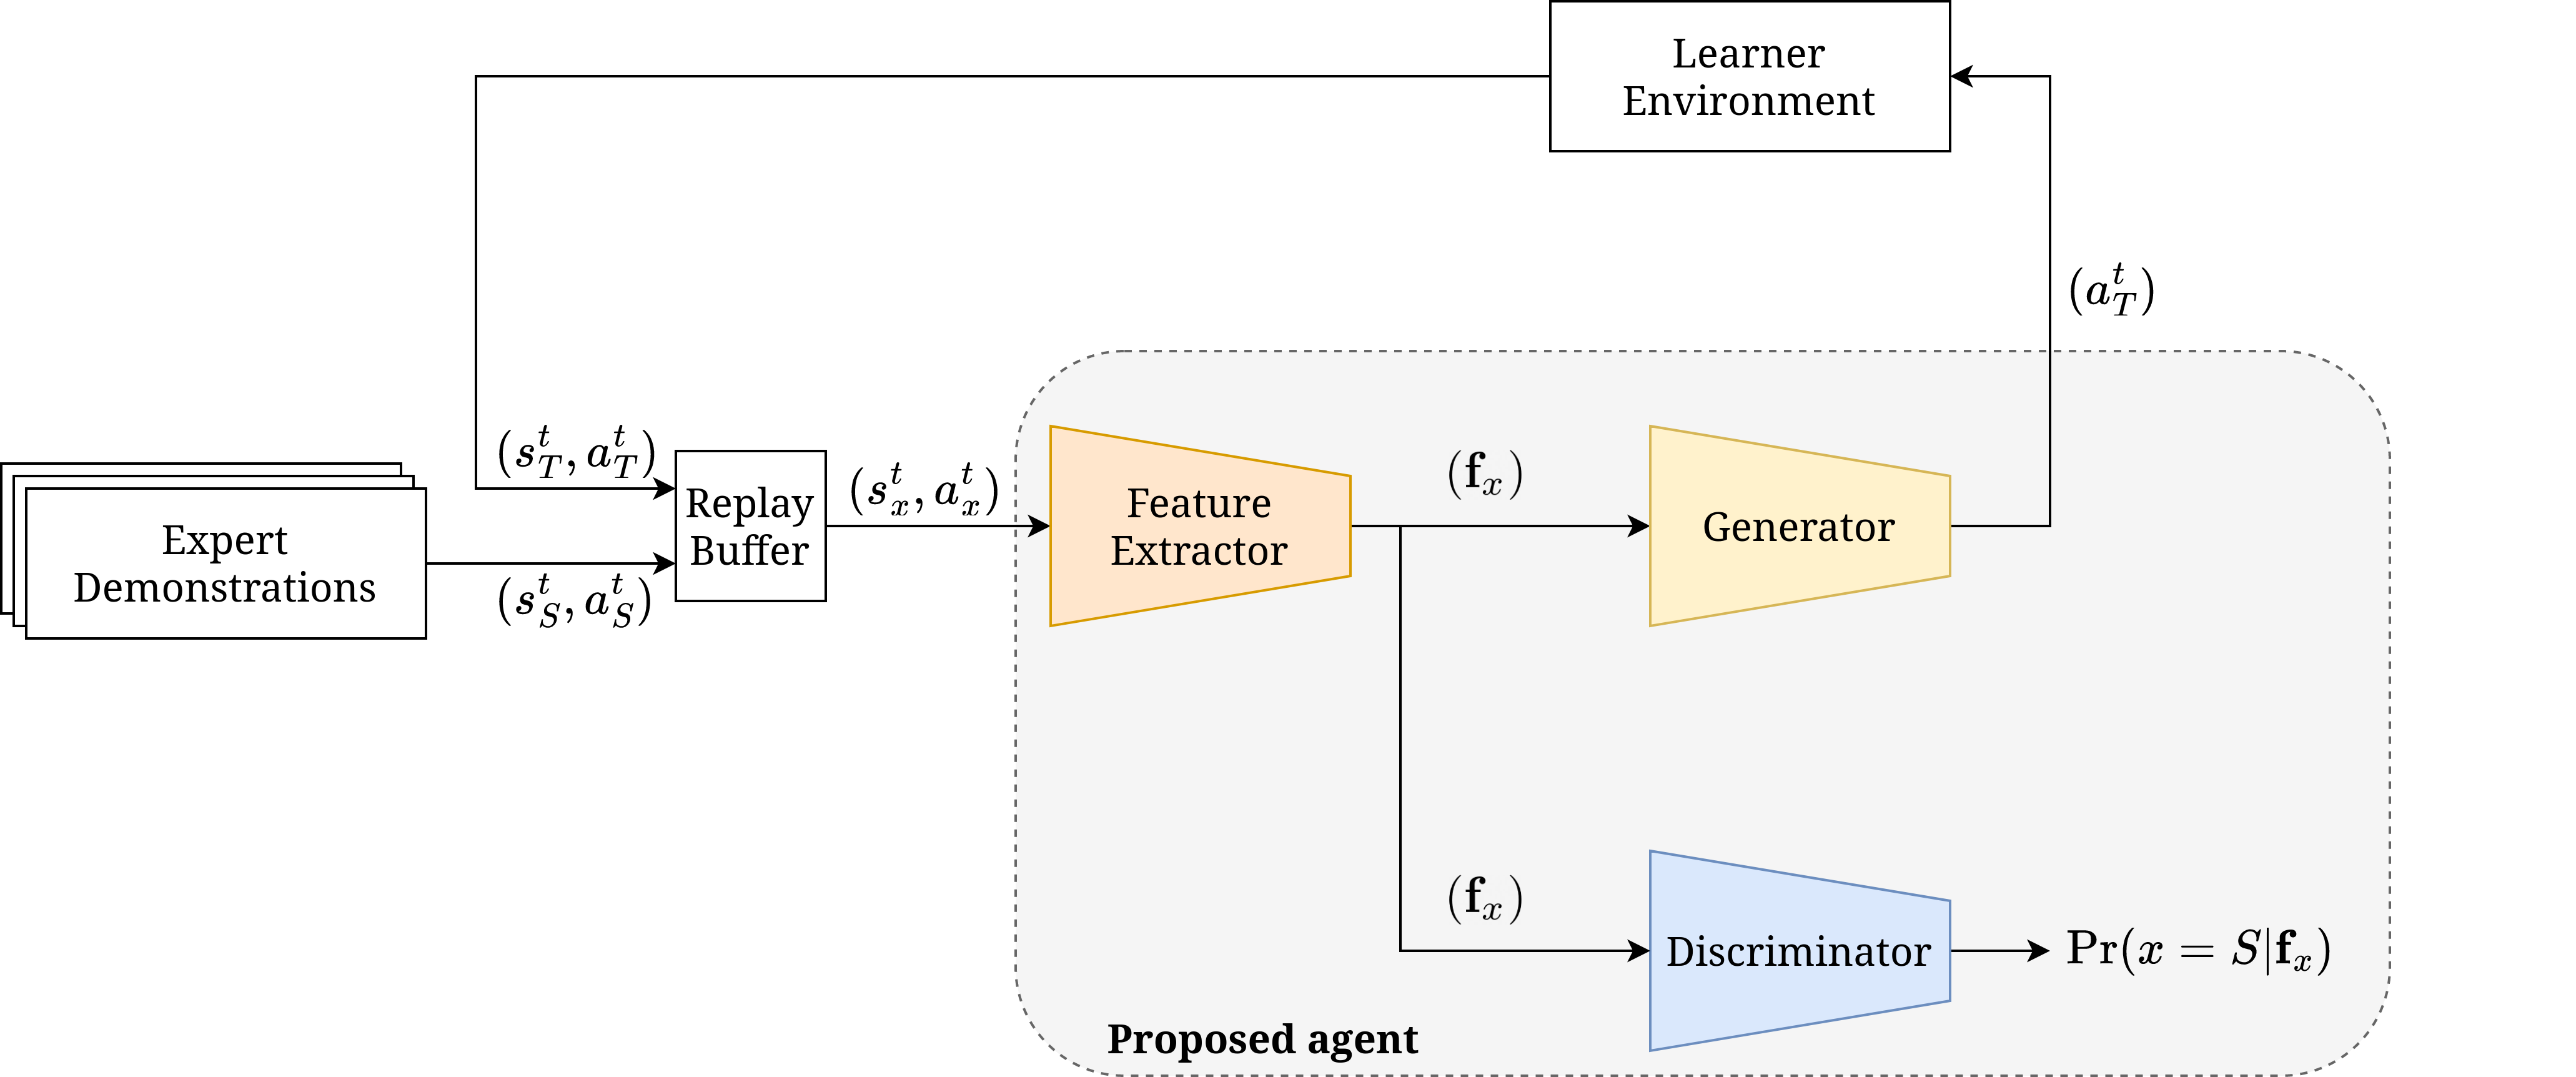
\includegraphics[width=0.9\linewidth]{\FigsDir/new_Architecture.png}
  \caption{\added{The neural network architecture of the proposed \TAIL{} agent.}\label{ch:TAIL:fig:Architecture}}
\end{figure}

\subsection{Feature Extractor Network \texorpdfstring{$F$}{F}}
A state-action pair $(s^t_x, a^t_x)$ in task $x$ is \added{sampled from a replay buffer \cite{zhang2017deeper} and} input to the feature extractor $F$ to produce a feature vector $\mathbf{f}_x=F(s^t_x, a^t_x)$.
$F$ is trained to capture the structural similarities or differences between source $\mathbb{M}^-_S$ and target $\mathbb{M}^-_T$ tasks by minimizing the distance between two features $\mathbf{f}_S$ and $\mathbf{f}_T$.
Therefore, the loss function of $F$ is defined as:

\begin{align}
  \mathfrak{L}_F (F, G) & = \mathbb{E} \left[ \left\|
    F(s^t_S, a^t_S) - F(s^t_T, a^t_T)
  \right\| \right]                                    \\
                        & = \mathbb{E} \left[ \left\|
    F(s^t_S, a^t_S) - F( s^t_T, G( F( s^t_S, a^t_S ) ) )
    \right\| \right]
  % 1/T \sum^{}_{}{|| f() - f() ||^2_2}
\end{align}


\subsection{Discriminator Network \texorpdfstring{$D$}{D} and Generator Network \texorpdfstring{$G$}{G}}

The discriminator $D$ is designed to distinguish between $\mathbf{f}_S$ and $\mathbf{f}_T$.
Specifically,
$D$ receives a feature vector $\mathbf{f}_x$ outputs a probability $\mathrm{Pr}(x=S|\mathbf{f}_x)$ to classify whether $\mathbf{f}_x$ is from source $\mathbb{M}^-_S$ or target $\mathbb{M}^-_T$ tasks.
Meanwhile,
the generator $G$ aims to generate an action $a^t_T$ so that $\mathbf{f}_T = F(s^t_T, a^t_T)$ looks as similar as possible to $\mathbf{f}_S$.
In the proposed \DAIL{} agent,
the adversarial loss \cite{GAN_Original} is applied for both networks:

\begin{align}
  \mathfrak{L}_{GAN}(G, D) & =
  \mathbb{E}[
    \log{D(F(s^t_S, a^t_S))}
  ] + \mathbb{E}[
    \log{(1-D(F(s^t_T, a^t_T)))}
  ]                                        \\
                           & = \mathbb{E}[
    \log{D(F(s^t_S, a^t_S))}
  ] + \mathbb{E}[
    \log{(1-D(F(s^t_T, G(F(
      s^t_S, a^t_S
      )))))}
  ]
\end{align}

The optimal policy is achieved using a RL-based policy gradient,
which relies on reward signal $r=-\log{D(F(s^t_S, a^t_S))}$ provided by the learned discriminator.


\subsection{Full Objective}

During the learning phase,
in order to capture the similarities and differences between source and target tasks,
the feature extractor $F$ and the generator $G$ are optimized to minimize the feature extractor loss $\mathfrak{L}_F$.
At the same time,
given a feature vector $\mathbf{f}_x$ of task $x$,
we want to judge whether $\mathbf{f}_x$ is from $\mathbb{M}^-_S$ or $\mathbb{M}^-_T$ by minimizing the task classification loss $\mathfrak{L}_{GAN}$.
This encourages task-specific features to be captured by $F$.
Overall, the full objective function is:

\begin{align}
   & \underset{F, G}{max} \underset{D}{min} \mathfrak{L}(F, G, D) \\
   & \quad\text{subject to \:}
  \mathfrak{L}(F, G, D) = {\mathfrak{L}_{GAN}(G, D)} - \lambda\mathfrak{L}_F
\end{align}

The learning algorithm of the proposed agent is outlined in Algorithm \ref{ch:TAIL:alg:ProposedModel}.

\begin{algorithm}
  \caption{\TAIL{}}
  \label{ch:TAIL:alg:ProposedModel}

  \begin{algorithmic}[1]
    \Input
    \Desc{$\mathcal{D}_\mathcal{S}$}{A set of expert demonstrations on source tasks}
    \EndInput

    \State Randomly initialize feature extractor network $F$, generator $G$ and discriminator $D$
    \For {i = 0, 1, 2, ...}
    \State Sample an expert demonstration $\tau^i_S \sim \mathcal{D}_S$
    \State Update the parameters of feature extractor network $F$ with the gradient
    \[\mathbf{E}[
        \nabla_F log(D( \mathbf{f}_S ))
      ] + \mathbf{E}[
        \nabla_F log(1 - D( \mathbf{f}_T ))
      ] - \lambda \mathbf{E}[
        \nabla_F \left\|
        \mathbf{f}_S - \mathbf{f}_T
        \right\|
      ]
    \]
    \State Update the discriminator parameters with the gradient
    \[\mathbf{E}[
        \nabla_D log(D( \mathbf{f}_S ))
      ] + \mathbf{E}[
        \nabla_D log(1 - D( \mathbf{f}_T ))
      ]\]
    \State Update policy $\pi_{L}$ with the reward signal $r=-logD(\mathbf{f}_S)$
    \EndFor

    \Output
    \Desc{$\pi_{T}$}{Learned policy for target task}
    \EndOutput
  \end{algorithmic}
\end{algorithm}


\section{Performance Evaluation\label{ch:TAIL:sec:Evaluation}}
In this section,
the performance of the proposed \TAIL{} is evaluated in comparison with baselines.
To support the evaluation,
different simulated tasks with varying difficulty levels ranging from simple to complex ones were utilized.
The details of these tasks are described in the next subsection.

\subsection{Experimental Settings}
\subsubsection{Simulated Tasks}


In order to examine the effectiveness of the proposed method,
six simulated tasks with varying difficulties were considered:
Pendulum \cite{Env_OpenAIGym},
CartPole \cite{Env_OpenAIGym, Env_CartPole},
WindowOpen \cite{Env_MetaWorld},
WindowClose \cite{Env_MetaWorld},
Door \cite{Env_Adroit},
and Hammer \cite{Env_Adroit}.
The task difficulty is varied along two axes;
the size of the state space and the size of the action space.
The detailed descriptions and visualizations of these tasks are shown in Table \ref{tab:Tasks} and Figure \ref{fig:Tasks}.
From such tasks,
three experiments were conducted,
each of which included two different tasks---a source task and a target task.
The detailed descriptions of these experiments are shown in Table \ref{tab:Experiments}.

\begin{landscape}

  \begin{table}[H]
    \caption{Description of six simulated tasks used in the experiment.\label{tab:Tasks}}

    \begin{tabular}{lcccp{5.5cm}}
      \toprule
      \textbf{Task}                               & \textbf{Size of State Space} & \textbf{Size of Action Space}                                              & \textbf{Difficulty Level} & \textbf{Description} \\
      \midrule
      Pendulum \cite{Env_OpenAIGym}               & 3 (continuous)               & 1 (continuous)
                                                  & Easy                         & Swinging up a pendulum.                                                                                                       \\
      CartPole \cite{Env_OpenAIGym, Env_CartPole} & 4 (continuous)               & 1 (continuous)
                                                  & Easy                         & Preventing the pendulum from falling over by applying a force to the cart.                                                    \\
      WindowOpen \cite{Env_MetaWorld}             & 39 (continuous)              & 4 (continuous)
                                                  & Medium                       & Opening a window.                                                                                                             \\
      WindowClose \cite{Env_MetaWorld}            & 39 (continuous)              & 4 (continuous)
                                                  & Medium                       & Closing a window.                                                                                                             \\
      Door \cite{Env_Adroit}                      & 39 (continuous)              & 28 (continuous)
                                                  & Hard                         & A 24-DoF hand attempts to undo the latch and swing the door open.                                                             \\
      Hammer \cite{Env_Adroit}                    & 46 (continuous)              & 26 (continuous)
                                                  & Hard                         & A 24-DoF hand attempts to use a hammer to drive the nail into the board.                                                      \\
      \bottomrule
    \end{tabular}
  \end{table}
\end{landscape}


\begin{figure}[H]
  \centering
  \begin{subfigure}[b]{0.2\textwidth}
    \centering
    \frame{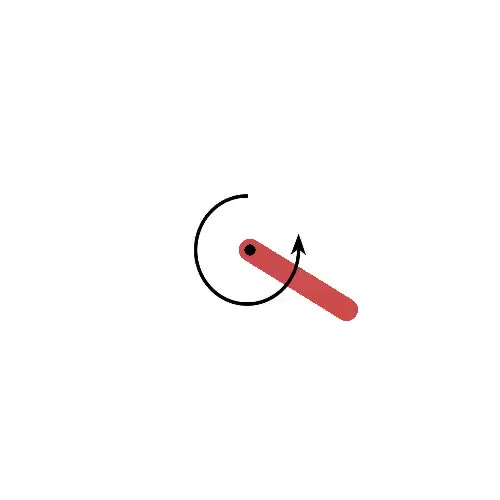
\includegraphics[width=\textwidth]{\FigsDir/Pendulum.jpg}}
    \caption{Pendulum}
  \end{subfigure}
  %
  \hfill
  %
  \begin{subfigure}[b]{0.2\textwidth}
    \centering
    \frame{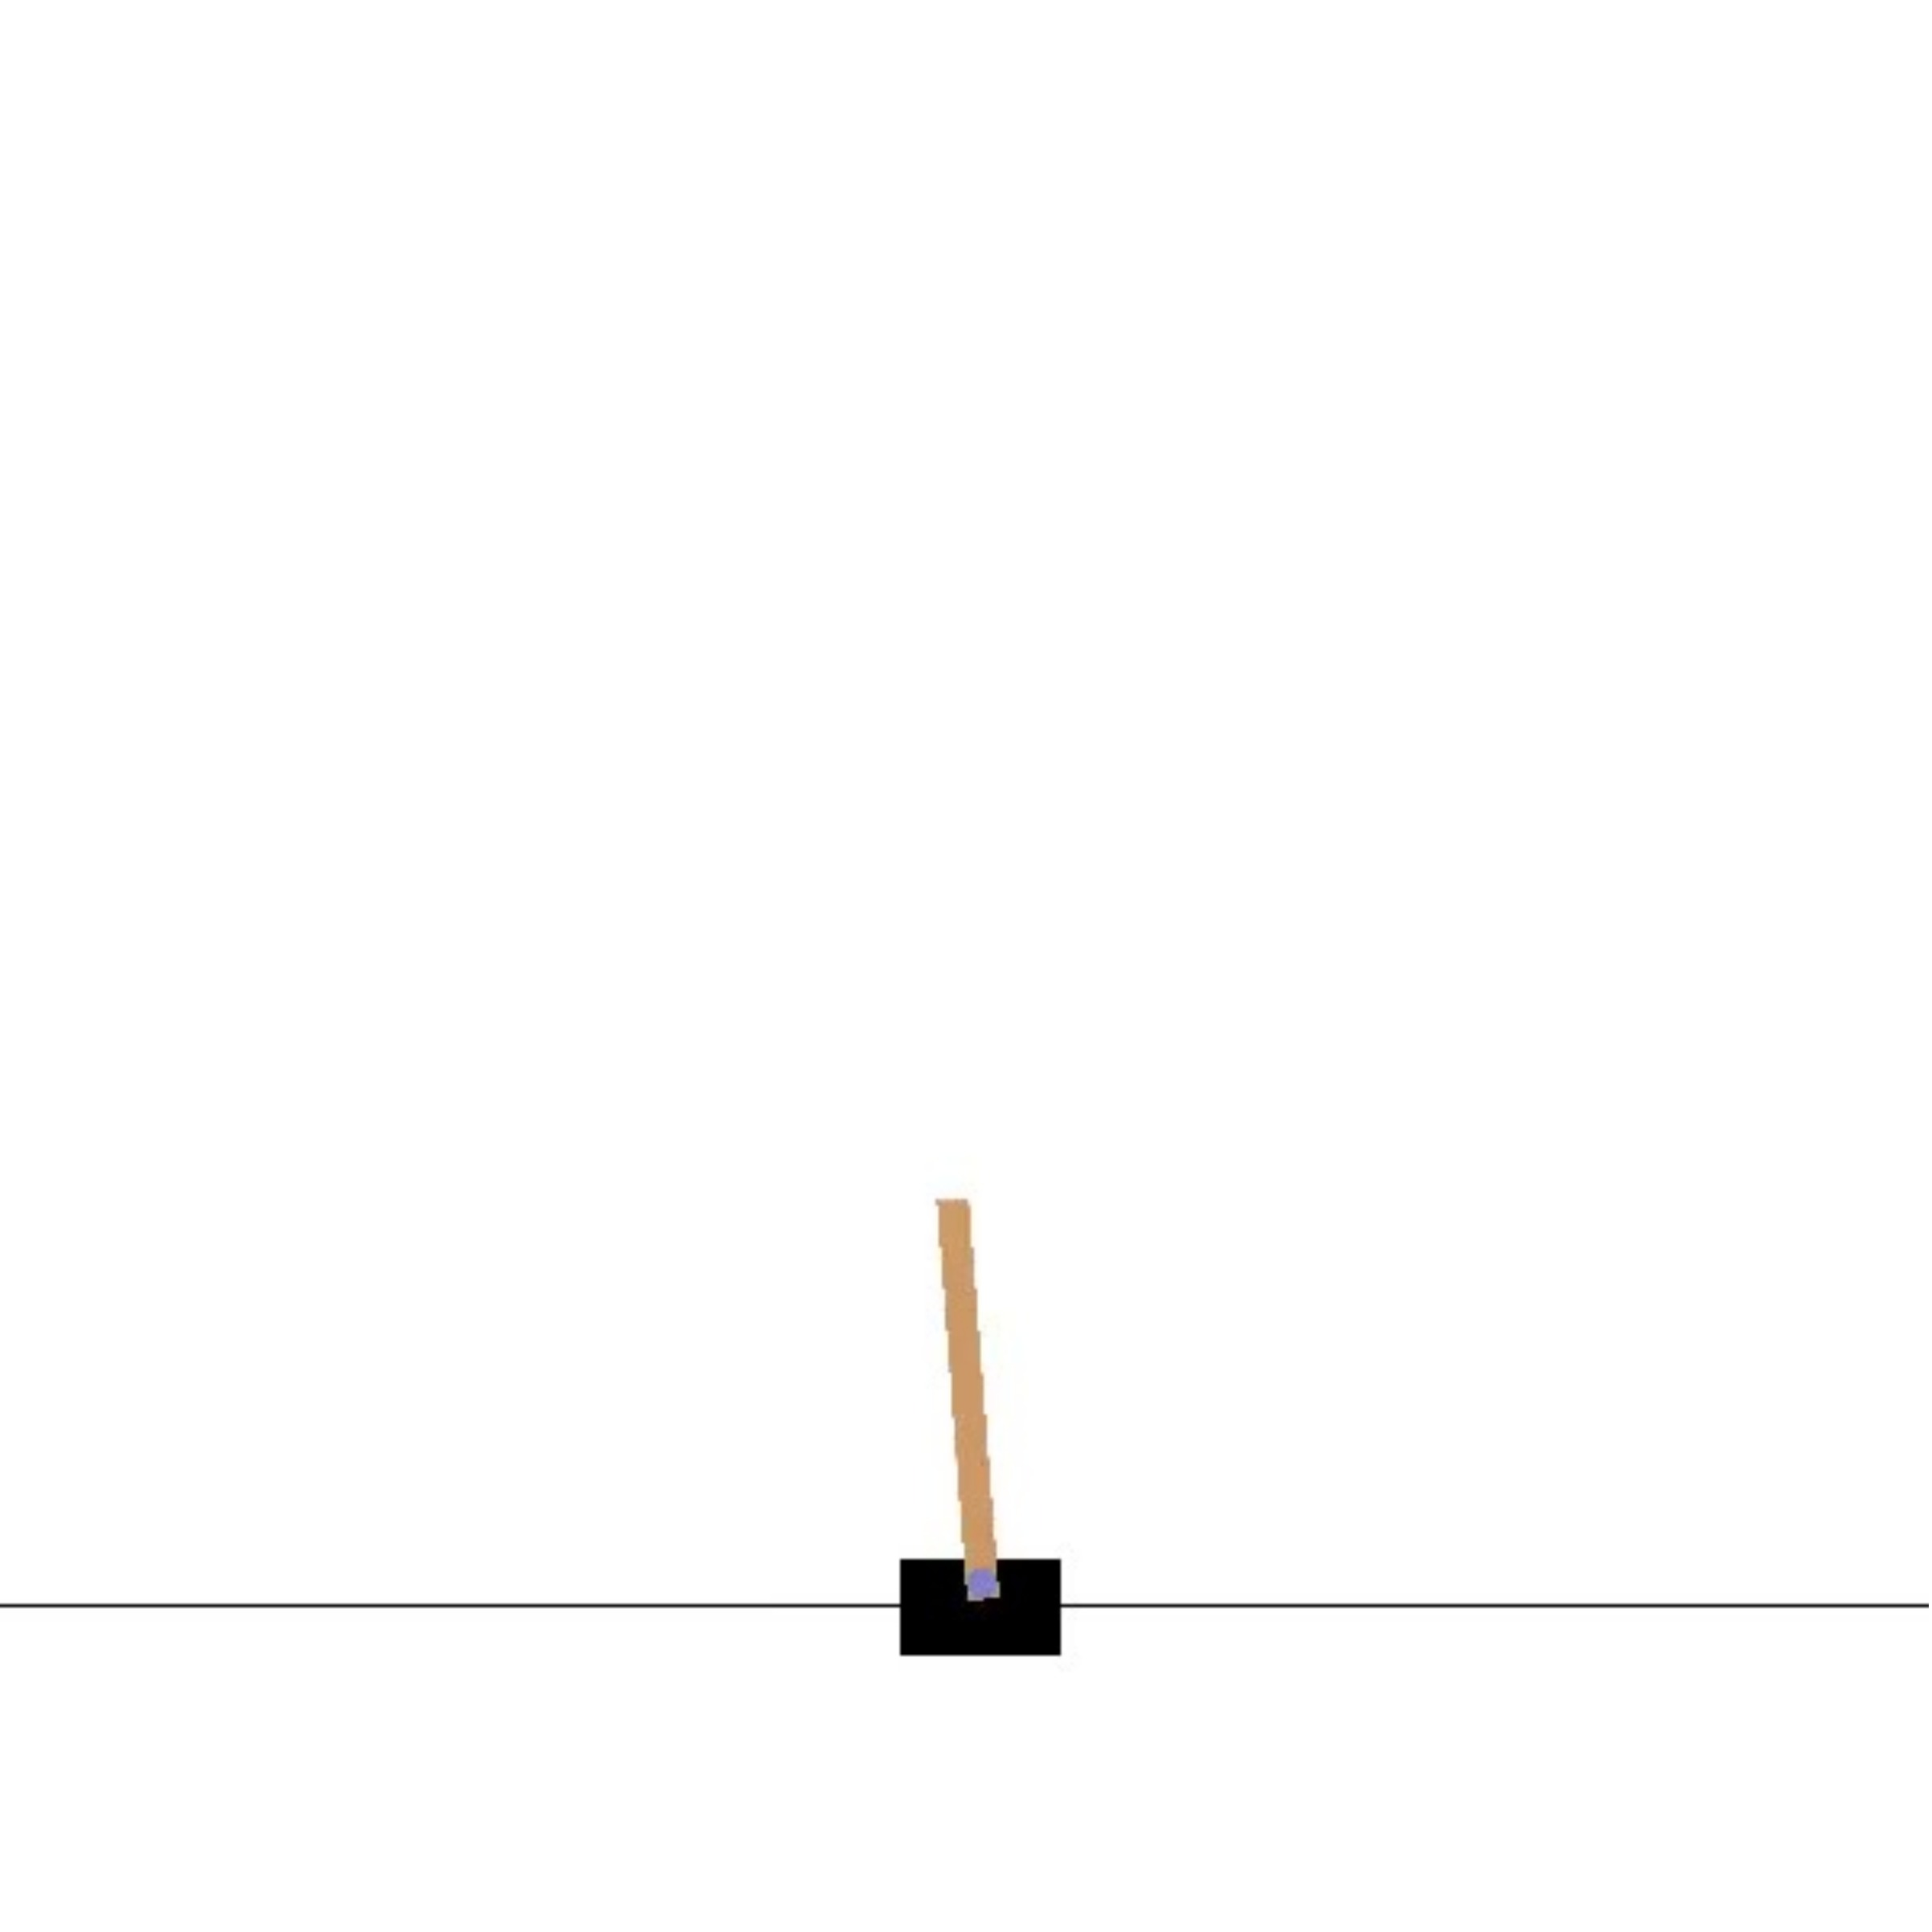
\includegraphics[width=\textwidth]{\FigsDir/CartPole.jpg}}
    \caption{CartPole}
  \end{subfigure}
  %
  \hfill
  %
  \begin{subfigure}[b]{0.25\textwidth}
    \centering
    \frame{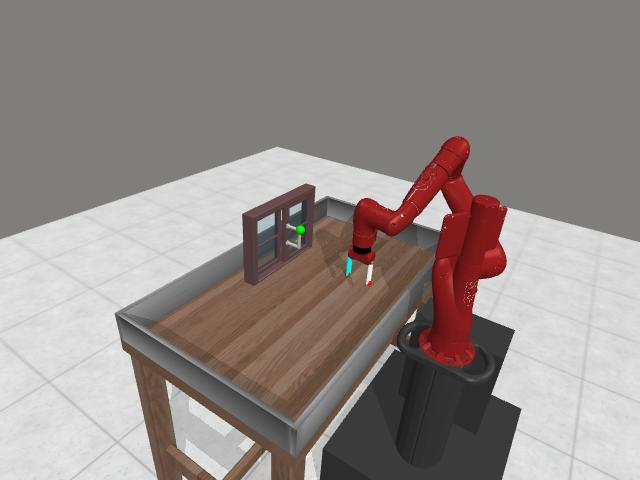
\includegraphics[width=\textwidth]{\FigsDir/WindowOpen.jpg}}
    \caption{WindowOpen}
  \end{subfigure}
  %
  \hfill
  %
  \begin{subfigure}[b]{0.25\textwidth}
    \centering
    \frame{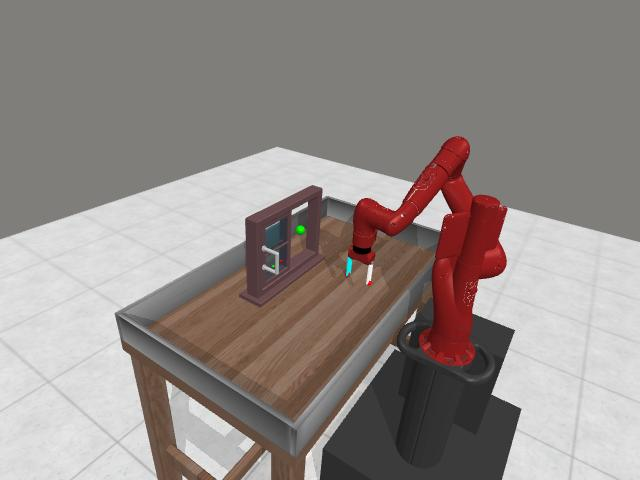
\includegraphics[width=\linewidth]{\FigsDir/WindowClose.jpg}}
    \caption{WindowClose}
  \end{subfigure}\\
  %
  \par\bigskip
  %
  \begin{subfigure}[b]{0.2\textwidth}
    \centering
    \frame{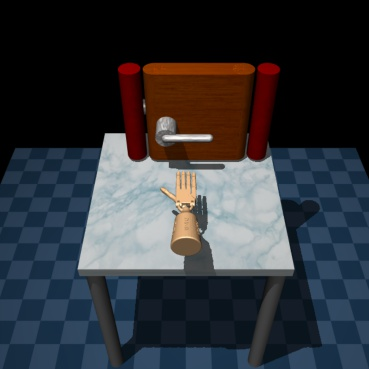
\includegraphics[width=\linewidth]{\FigsDir/Door.jpg}}
    \caption{Door}
  \end{subfigure}
  %
  % \hfill
  %
  \hspace{4em}
  \begin{subfigure}[b]{0.2\textwidth}
    \centering
    \frame{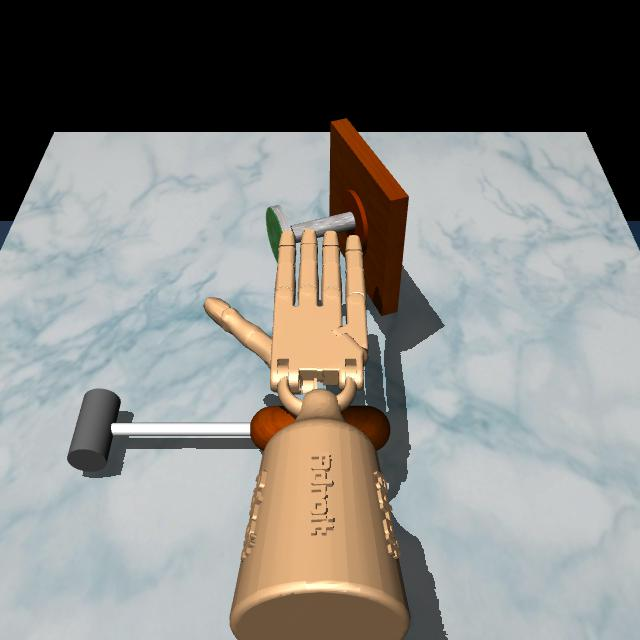
\includegraphics[width=\linewidth]{\FigsDir/Hammer.jpg}}
    \caption{Hammer}
  \end{subfigure}
  %
  \caption{Visual rendering of five simulated tasks used in the experiment.\label{fig:Tasks}}
\end{figure}
\unskip

\begin{landscape}
  \begin{table}[H]
    \centering
    \caption{Description of three experiments conducted to evaluate the performance of the proposed method.\label{tab:Experiments}}

    \begin{tabular}{lcccp{5.5cm}}
      \toprule
      \textbf{Experiment}     & \textbf{Source Task} & \textbf{Target Task}                                                                               & \textbf{Difficulty Level} & \textbf{Description} \\
      \midrule
      Pendulum--CartPole      & Pendulum             & CartPole
                              & Easy                 & A simple experiment in which both source and target tasks have small state and action spaces.                                                         \\
      WindowOpen--WindowClose & WindowOpen           & WindowClose
                              & Medium               & Both source and target tasks have a large state space but small action space.                                                                         \\
      Door--Hammer            & Door                 & Human
                              & Hard                 & A challenging experiment in which both source and target tasks have large state and action spaces.                                                    \\
      \bottomrule
    \end{tabular}
  \end{table}
\end{landscape}

In order to train and adapt the proposed \TAIL{} agent,
expert demonstrations for both source and target tasks must be provided.
In this experiment,
the proximal policy optimization (PPO) method was chosen to be trained on each task in order to create an expert RL agent.
The reason behind this decision was that PPO was recently showing the best result for many complex tasks.
After that,
the demonstrations were collected by executing the trained PPO expert agent in the simulated task.
For the source task, 30 demonstrations were collected to provide sufficient data for training the proposed agent \cite{IL_Model_GAIL}.
In the adaptation process, the proposed agent already learned the knowledge of the source task, thus, a smaller number of demonstrations for the target task is required.
Therefore, only 15 demonstrations were collected for the target task.


%==================================================
\subsubsection{Baselines}


To evaluate the performance of the proposed agent,
two baselines were considered.
\begin{description}
  \item[PPO + Fine-tuning]
        The agent is trained on the source task using Proximal Policy Optimization (PPO) \cite{Baseline_PPO}, which is a policy optimization method.
        Then, fine-tuning is applied to adapt the trained agent to the target task.
        Fine-tuning is a common transfer learning technique that simply re-trains the agent on a new target task.

  \item[NFQI + TA-TL]
        NFQI + TA-TL is a policy adaptation method, where first it utilizes  Neural Fitted Q-iteration (NFQI) \cite{Baseline_NFQI} to find an optimal policy on a source task,
        then that policy is transferred to a new target task.
        NFQI is a Q-learning method that tries to estimate the Q-function using a deep feed-forward network.
\end{description}

In order to provide a fair comparison,
each baseline was evaluated for 100 trials.
The success rate and average cumulative reward were used as performance metrics.
The success rate indicates the percentage of trials in which the baseline can successfully complete a task.
The average cumulative reward measures how well the baseline performed in a trial.

\subsection{Results}

The result is tabulated in Table \ref{ch:TAIL:tab:Result_SuccessRate_After_Target}.
The behavior of those agents when performing target tasks is visualized in Figure \ref{fig:Result_After_Target}.
It can be seen that the proposed \TAIL{} and baselines provide comparably similar behaviors in order to solve target tasks.
This result indicated that the proposed agent successfully adapted and transferred the agent's knowledge to the new target task.
Moreover, it can be observed from Table \ref{ch:TAIL:tab:Result_SuccessRate_After_Target} that \TAIL{} outperformed other baselines.
In addition, it performed highly well and consistently on the complex WindowClose and Hammer tasks.
Applying fine tuning to the PPO agent also provided a consistent performance across all three tasks.
At the same time, applying TA-TL to the NFQI agent was not able to produce a high success rate due to the high complexity of the WindowClose and Hammer tasks.


The results demonstrated that the proposed agent not only outperformed baselines in terms of success rate on all target tasks, but notably produced a consistently high performance, even on the most difficult task.
This proved the potential of the proposed agent and adversarial learning in order to tackle the task adaptation problem in imitation learning.

\begin{table}[H]
  \footnotesize
  \caption{The performance of the proposed agent on target tasks after adaptation. \label{ch:TAIL:tab:Result_SuccessRate_After_Target}}

  \centering
  \setlength{\tabcolsep}{.7mm}{\begin{tabular}{llccc}
      \toprule
       &                                       & \textbf{CartPole} & \textbf{WindowClose} & \textbf{Hammer}       \\
      \midrule
      \multirow{4}{*}{Success rate}
       & \TAIL{}                               & 100\%             & 85\%                 & 80\%                  \\
       & PPO \cite{Baseline_PPO} + Fine-tuning & 100\%             & 82\%                 & 76\%                  \\
       & NFQI + TA-TL \cite{Baseline_TATL}     & 100\%             & 77\%                 & 70\%                  \\
      \midrule
      \multirow{4}{*}{Average cumulative reward}
       & \TAIL{}                               & $500.00 \pm 0.0$  & $2473.10 \pm 619.13$ & $3351.69 \pm 1957.30$ \\
       & PPO \cite{Baseline_PPO} + Fine-tuning & $500.00 \pm 0.0$  & $2402.65 \pm 638.54$ & $3165.05 \pm 1134.02$ \\
       & NFQI + TA-TL \cite{Baseline_TATL}     & $500.00 \pm 0.0$  & $1457.53 \pm 621.37$ & $2840.35 \pm 1036.76$ \\
      \bottomrule
    \end{tabular}}
\end{table}



\begin{landscape}
  \begin{figure}[H]
    \centering
    %
    \begin{subfigure}[b]{\linewidth}
      \centering
      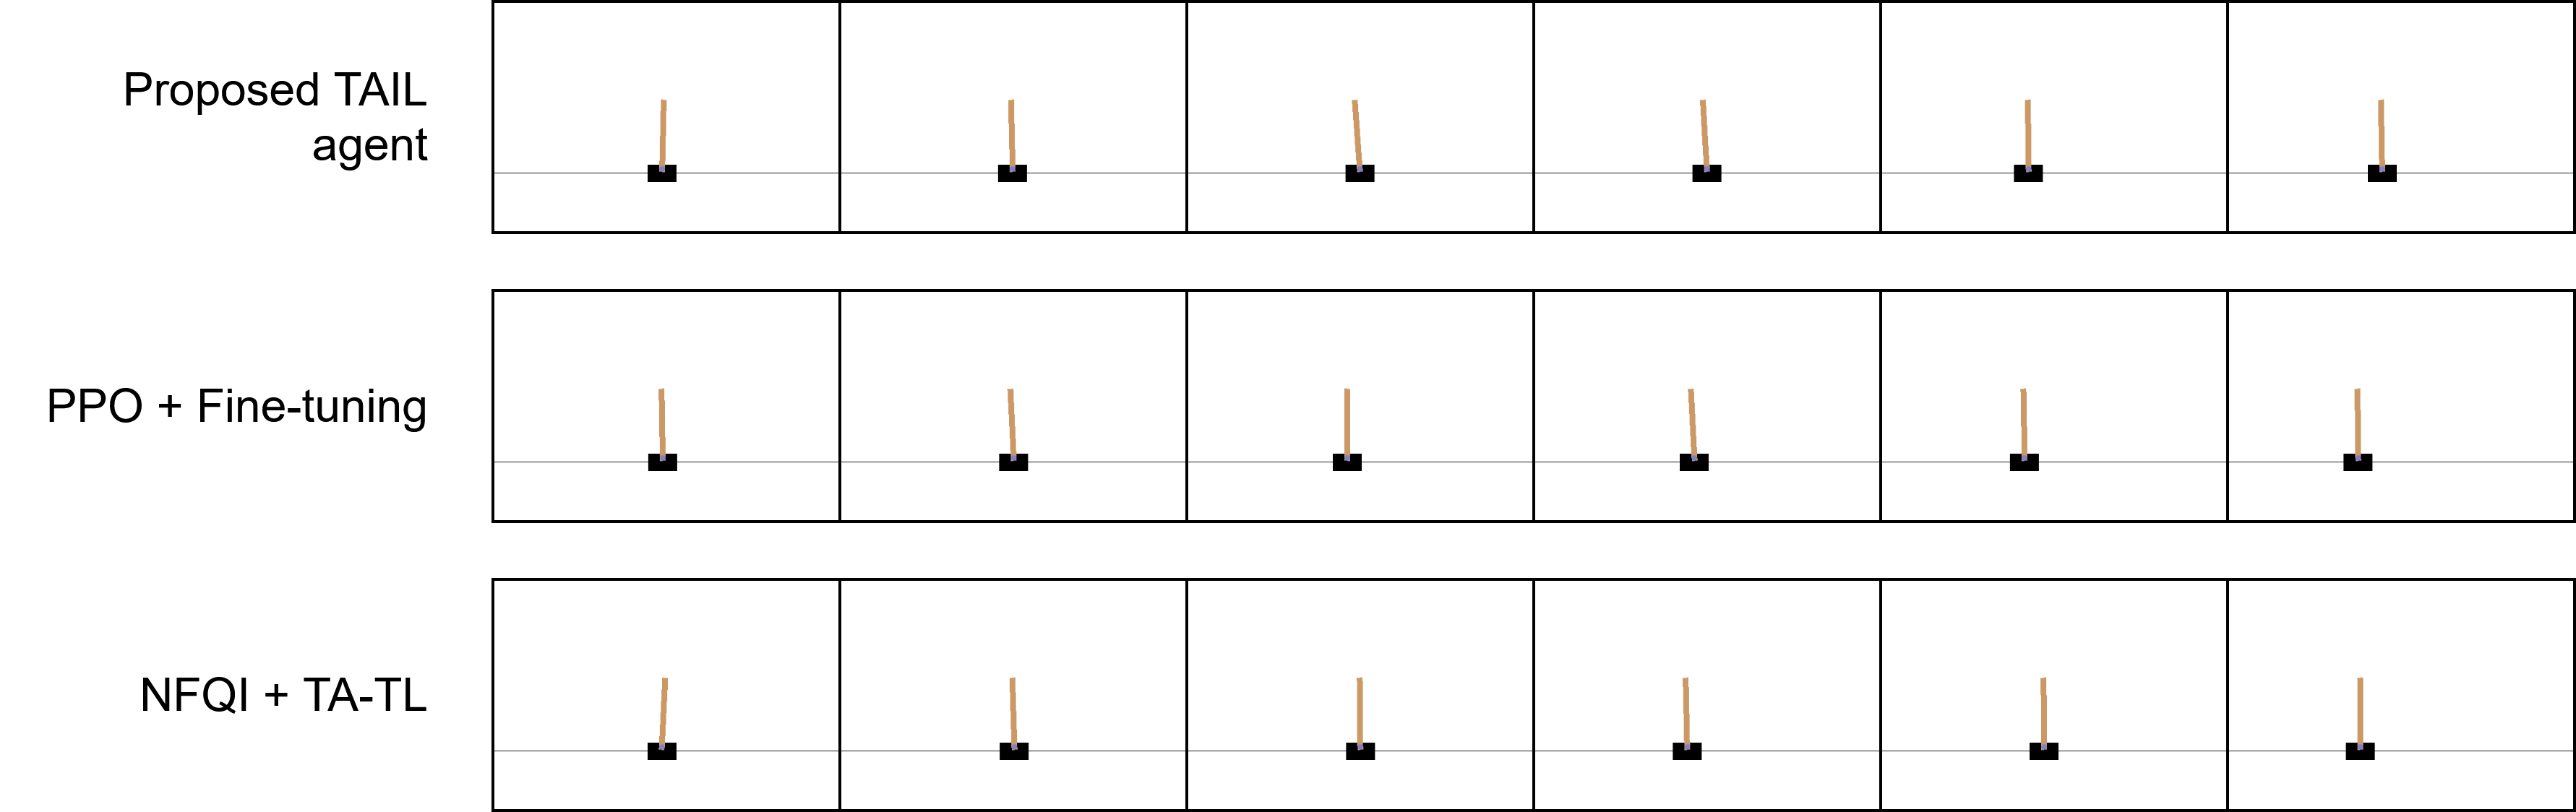
\includegraphics[width=\linewidth]{\FigsDir/Result_After_CartPole.png}
      \caption{\centering CartPole}
    \end{subfigure}
    %
    \par\bigskip
    %
    \begin{subfigure}[b]{\linewidth}
      \centering
      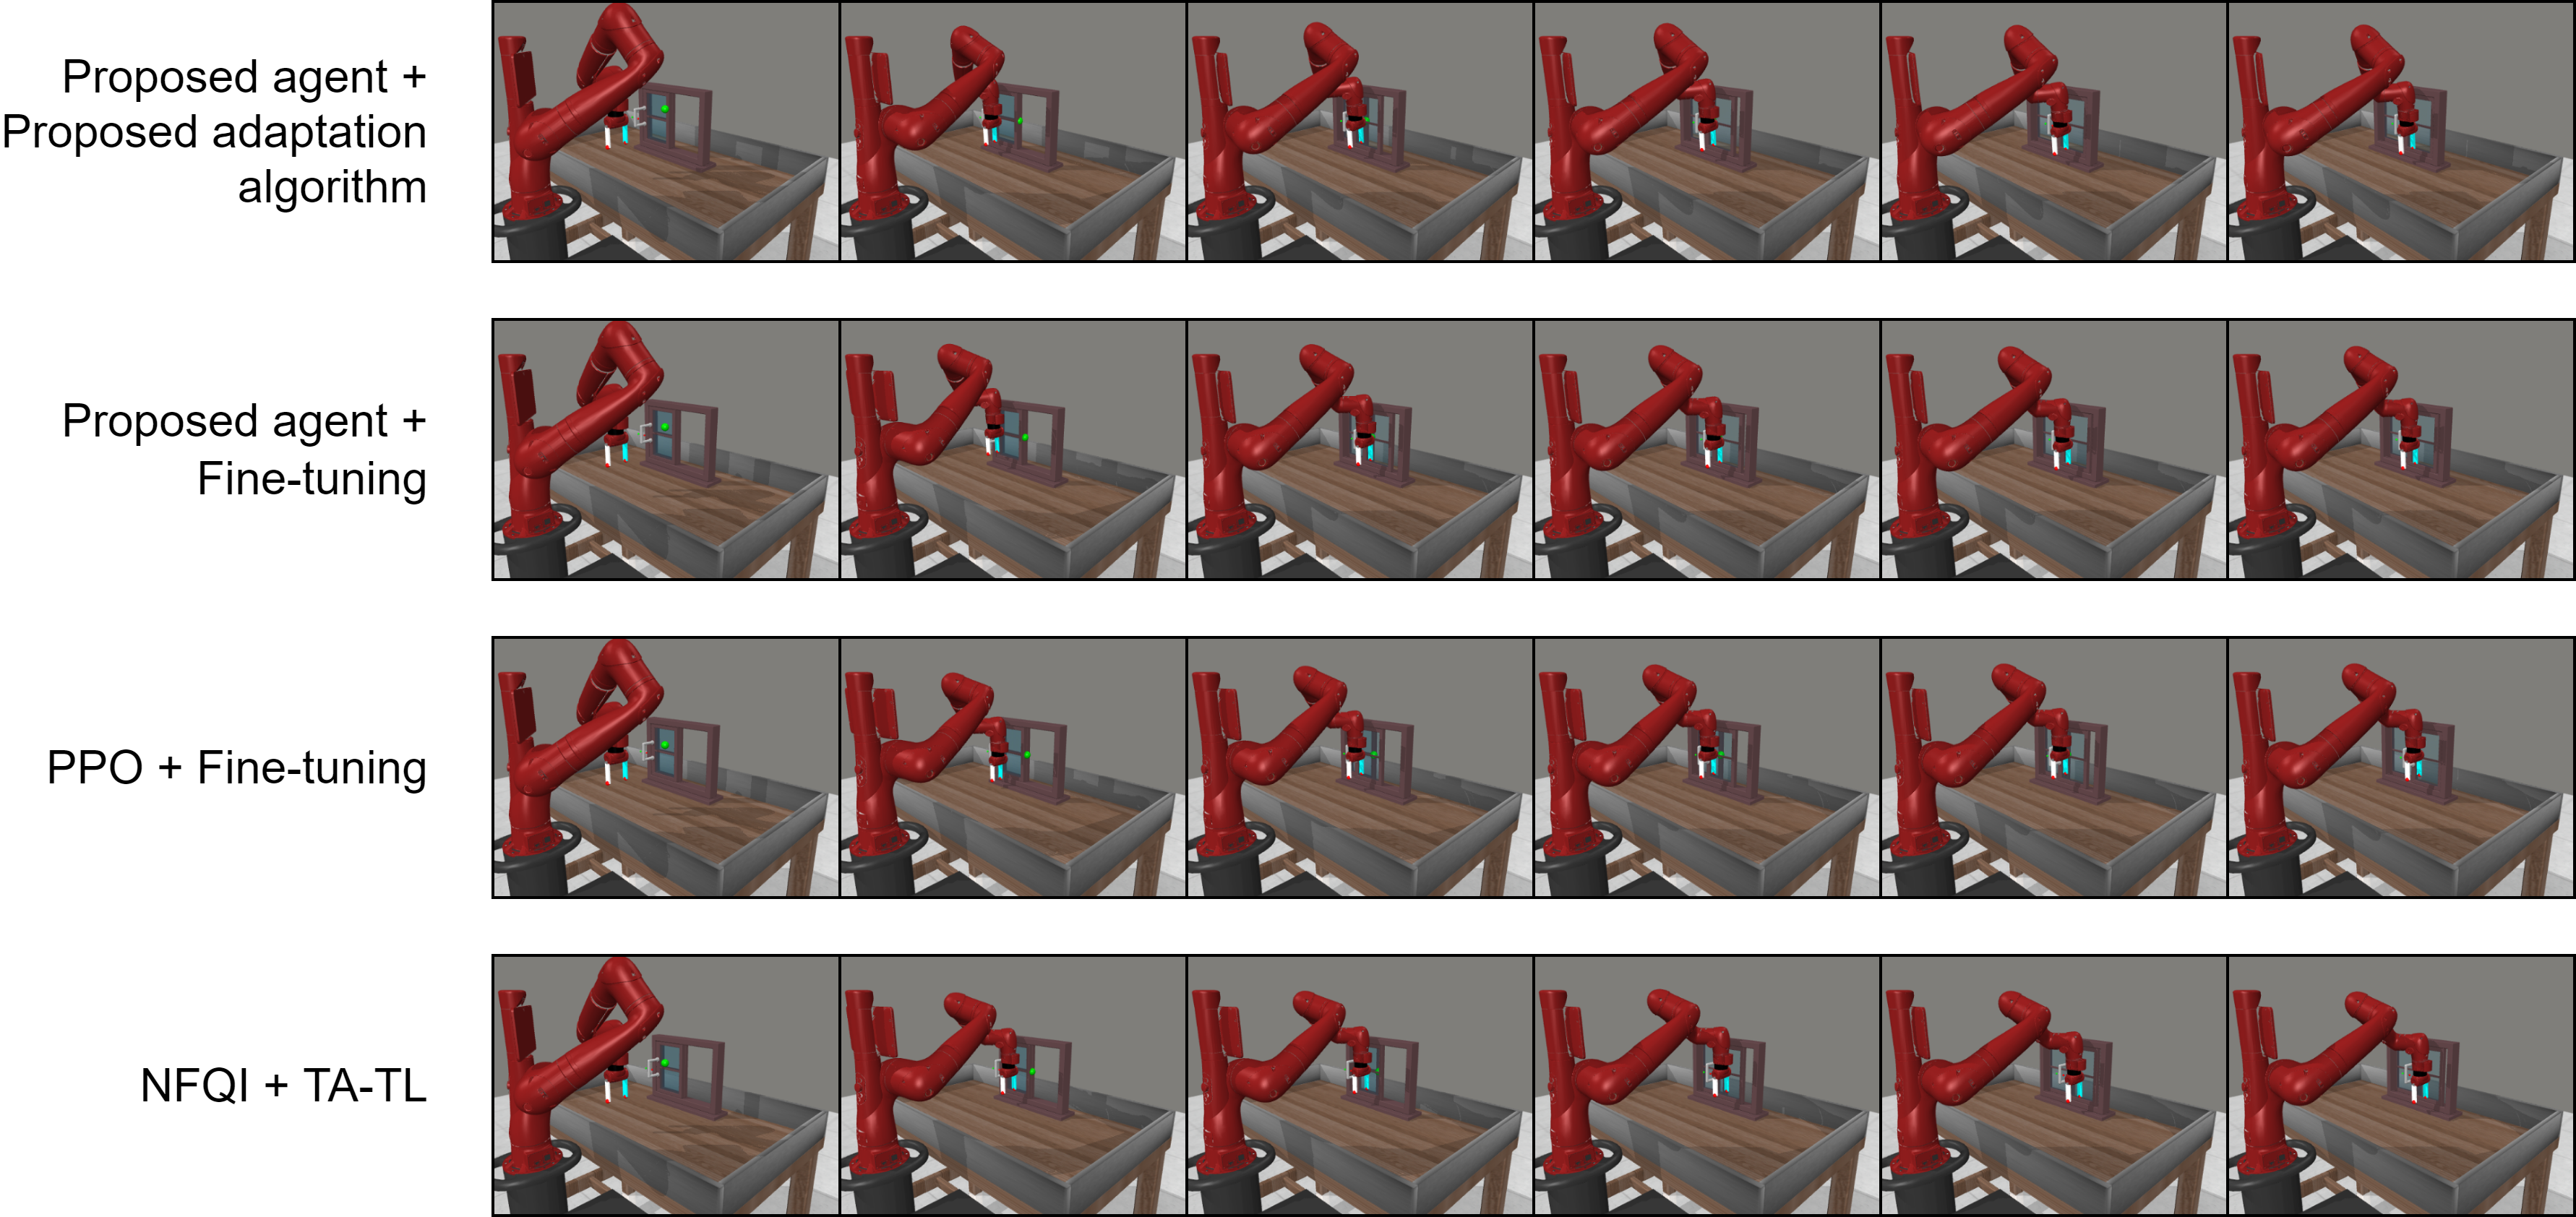
\includegraphics[width=\linewidth]{\FigsDir/Result_After_WindowClose.png}
      \caption{\centering WindowClose}
    \end{subfigure}
    %
    \caption{\textit{Cont}.}
  \end{figure}
  \begin{figure}[H]\ContinuedFloat
    \centering
    %
    \begin{subfigure}[b]{\linewidth}
      \centering
      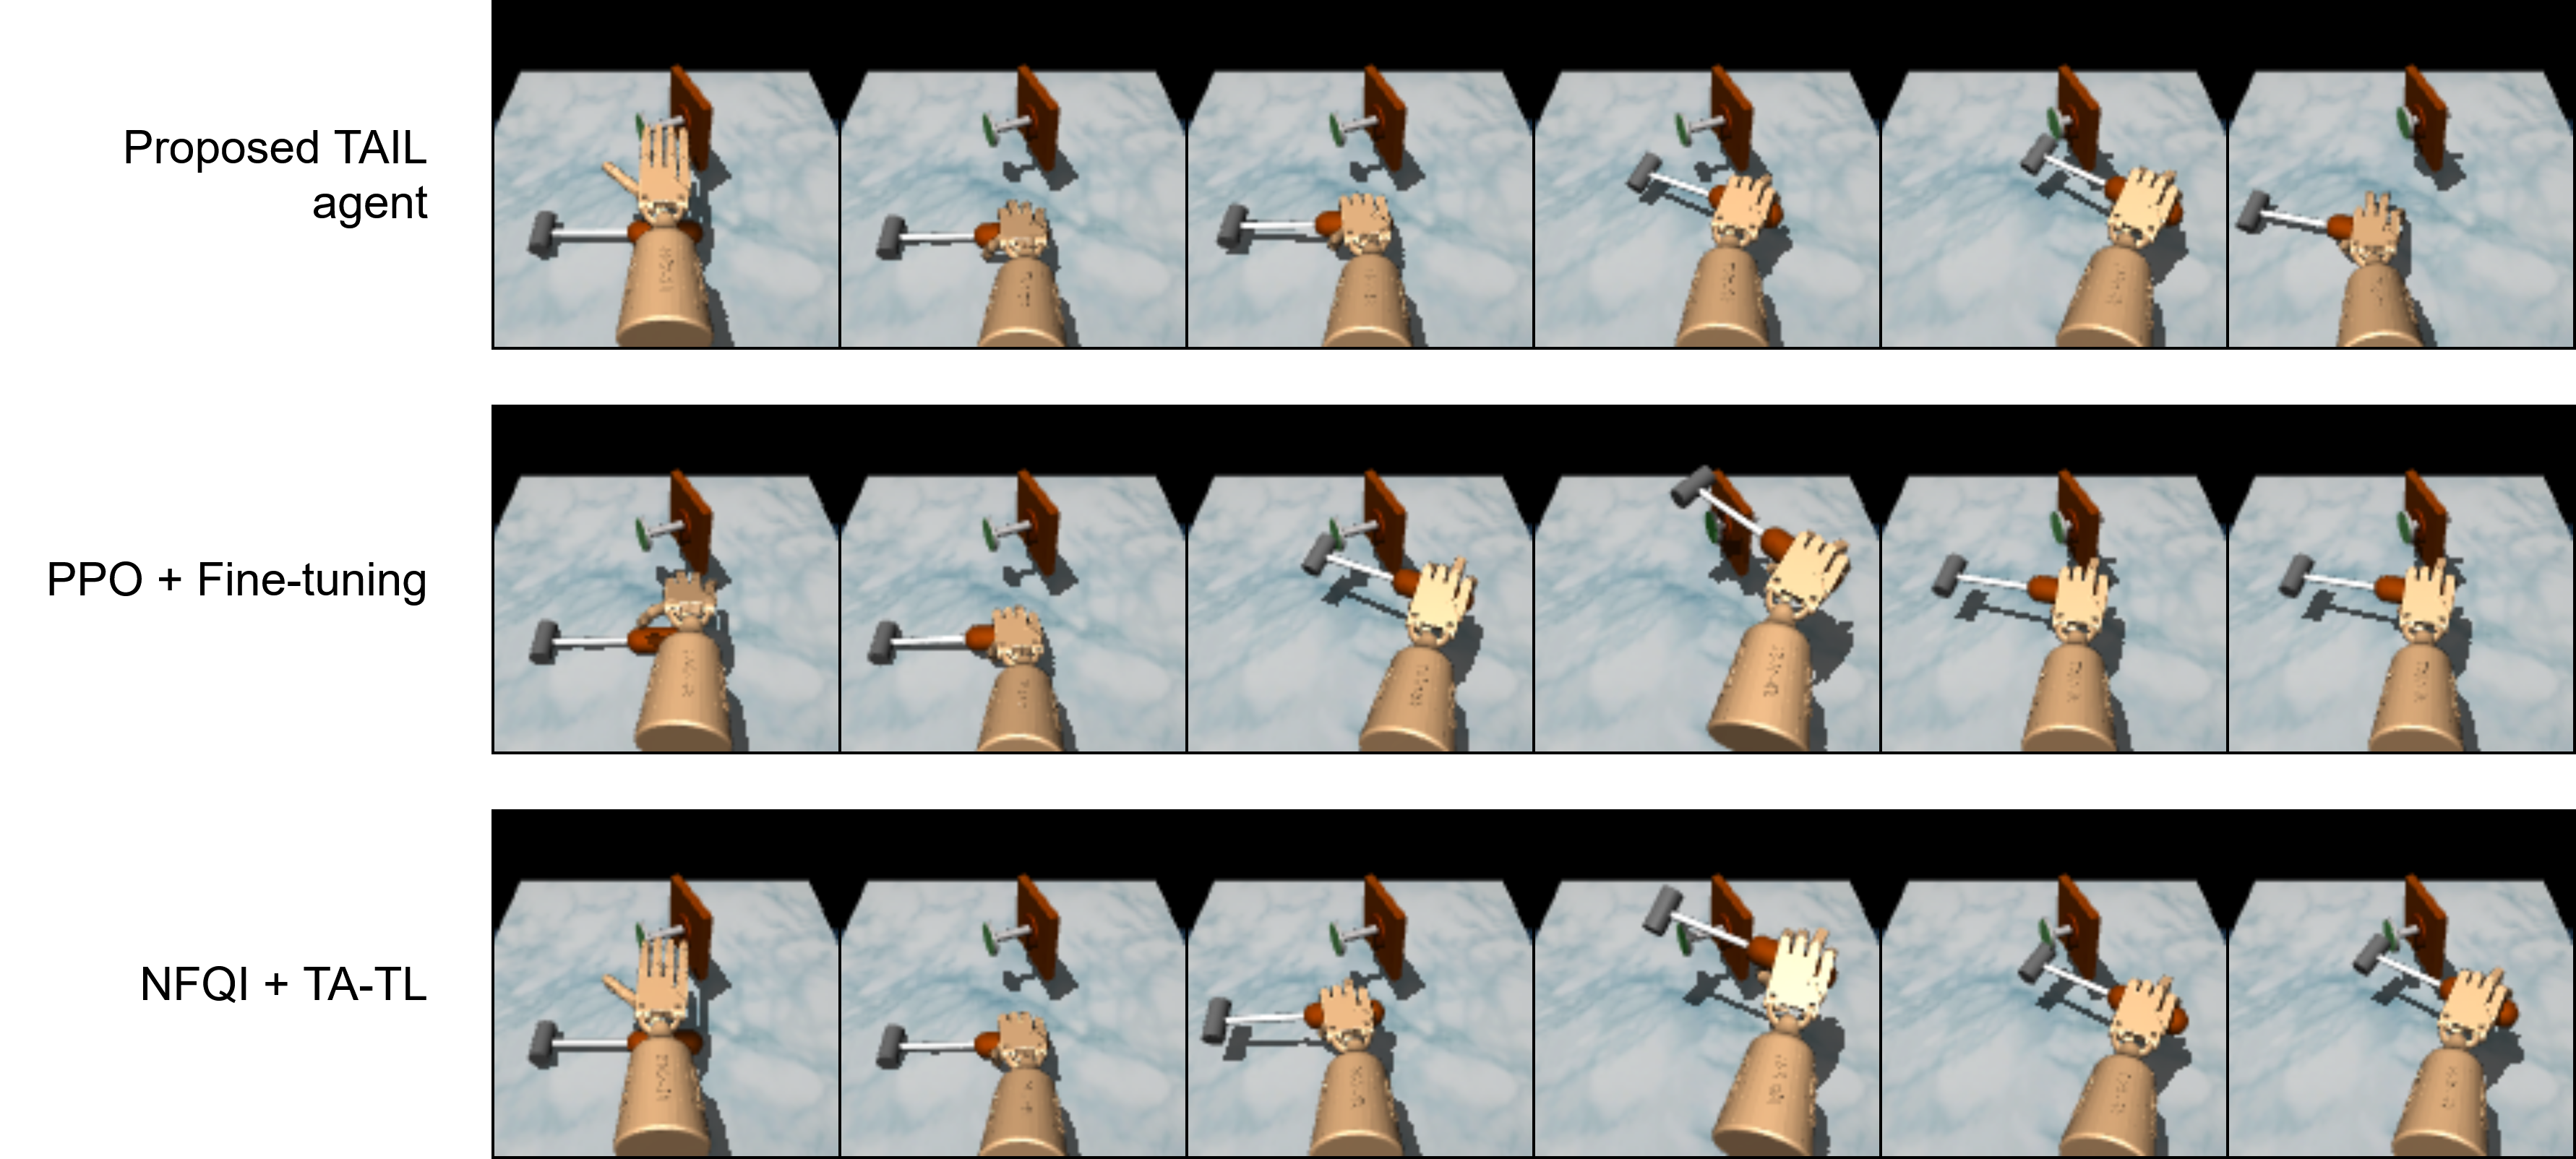
\includegraphics[width=\linewidth]{\FigsDir/Result_After_Hammer.png}
      \caption{\centering Hammer}
    \end{subfigure}
    %
    \caption{A visualization of the behavior of the proposed agent and baselines on target tasks.\label{fig:Result_After_Target}}
  \end{figure}
  \unskip
\end{landscape}

% \subsubsection{Computational Complexity}
% Besides evaluating the performance of the proposed agent in terms of success rate,
% its computational cost was also assessed in order to provide an adequate study of its overall performance.
% Table \ref{tab:Result_Cost} shows the training time required to train the agent in each experiment.
% It can be observed that the training time when applying fine tuning to PPO was slightly better than the training time of the proposed adaptation method,
% especially on two complex WindowOpen-WindowClose and Door--Hammer experiments.
% On the other hand, compared to TA-TL, the proposed adaptation method required a higher training time on all three experiments.
% This result was expected since,
% during the proposed adaptation process,
% the agent had to not only learn the new task, but also review the previously learned source task.
% However,
% it should be noted that the training time of the proposed adaptation method can be further improved by leveraging the parallel training process \cite{DL_Lib_StableBaselines3, DL_Lib_Tianshou}.


% \begin{table}[H]
%   \caption{The training time (s/epoch) of the proposed agent.\label{tab:Result_Cost}}

%   \centering
%   \begin{tabular}{lccc}
%     \toprule
%                                           & \textbf{Pendulum--CartPole} & \textbf{WindowOpen--WindowClose} & \textbf{Door--Hammer} \\
%     \midrule
%     \TAIL{}                               & 86.623                      & 165.768                          & 538.790               \\
%     PPO \cite{Baseline_PPO} + Fine-tuning & 84.234                      & 164.472                          & 534.234               \\
%     NFQI + TA-TL \cite{Baseline_TATL}     & 68.329                      & 129.420                          & 492.059               \\
%     \bottomrule
%   \end{tabular}
% \end{table}


\section{Discussion\label{ch:TAIL:sec:Discussion}}
In this section,
the effects of adversarial learning on training the \TAIL{} agent are discussed in detail.

The experimental results assessed in the previous section have shown the potential of \TAIL{} in tackling the task adaptation problem in imitation learning.
As shown in Tables \ref{ch:TAIL:tab:Result_SuccessRate_After_Target},
\TAIL{} could provide consistent and high performance in terms of success rate target tasks with varying difficulty levels.
This promising result demonstrates the effectiveness of applying adversarial learning,
in which the agent can extract the similarities and differences between source and target tasks to adapt its learned knowledge effectively.
Although the performance of \TAIL{} remained limited,
it has demonstrated the potential of adversarial learning in improving generalization in imitation learning.


\section{Summary}
In this chapter, the \TAIL{} agent was proposed to tackle the task adaptation problem in imitation learning.
The experimental results demonstrated that the agent was able to extract the similarity and differences between source and target tasks in order to provide high performance on the target task in terms of success rate.

